\section{Lab 3}

\begin{frame}
   {Device Tree}

   In Lab3, we will accomplish the following:
	\begin{itemize}
		\item
			Learn Pocketbeagle DT specifics
		\item
			Configure the platform DT for our joystick device
		\item
			Overlay the base DT with the joystick device
	\end{itemize}
\end{frame}

\begin{frame}
	{pocketbeagle.dts P1.29 pinctrl node}

	\begin{raw}
	/* P1_29 (ZCZ ball A14) pruin */
	P1_29_pinmux {
		compatible = "bone-pinmux-helper";
		status = "okay";
		pinctrl-names = "default", "gpio", "gpio_pu", "gpio_pd",
				"gpio_input", "qep", "pruout", "pruin";
		pinctrl-0 = <&P1_29_default_pin>;
		pinctrl-1 = <&P1_29_gpio_pin>;
		pinctrl-2 = <&P1_29_gpio_pu_pin>;
		pinctrl-3 = <&P1_29_gpio_pd_pin>;
		pinctrl-4 = <&P1_29_gpio_input_pin>;
		pinctrl-5 = <&P1_29_qep_pin>;
		pinctrl-6 = <&P1_29_pruout_pin>;
		pinctrl-7 = <&P1_29_pruin_pin>;
	};
	\end{raw}
\end{frame}

\begin{frame}
	{pocketbeagle.dts P2.33 pinctrl node}

	\begin{raw}
/* P2_33 (ZCZ ball R12) */
	P2_33_pinmux {
		compatible = "bone-pinmux-helper";
		status = "okay";
		pinctrl-names = "default", "gpio", "gpio_pu", "gpio_pd",
				"gpio_input", "qep", "pruout";
		pinctrl-0 = <&P2_33_default_pin>;
		pinctrl-1 = <&P2_33_gpio_pin>;
		pinctrl-2 = <&P2_33_gpio_pu_pin>;
		pinctrl-3 = <&P2_33_gpio_pd_pin>;
		pinctrl-4 = <&P2_33_gpio_input_pin>;
		pinctrl-5 = <&P2_33_qep_pin>;
		pinctrl-6 = <&P2_33_pruout_pin>;
	};
	\end{raw}
\end{frame}

\begin{frame}
	{P1.29 GPIO resource}

	\url{http://www.ti.com/lit/ds/symlink/am3352.pdf}

	     \begin{figure}[H]
		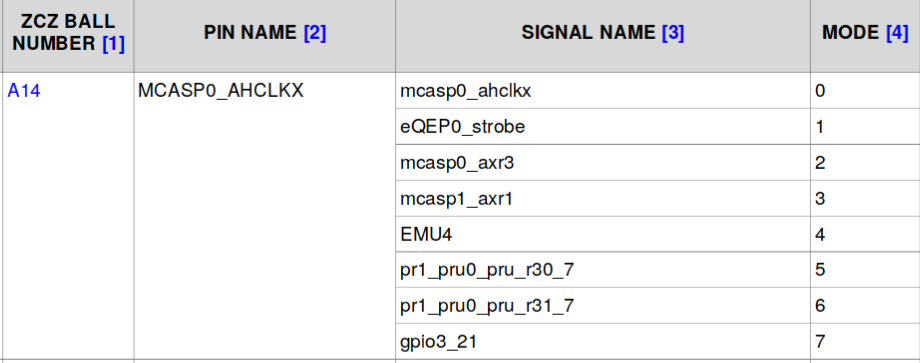
\includegraphics[width=5in]{IMAGES/p129-zcz-a14}
		     \caption{P1.29 ZCZ A14 (gpio3\_21)}
	     \end{figure}
\end{frame}

\begin{frame}
	{P2.33 GPIO resource}

	\url{http://www.ti.com/lit/ds/symlink/am3352.pdf}

	     \begin{figure}[H]
		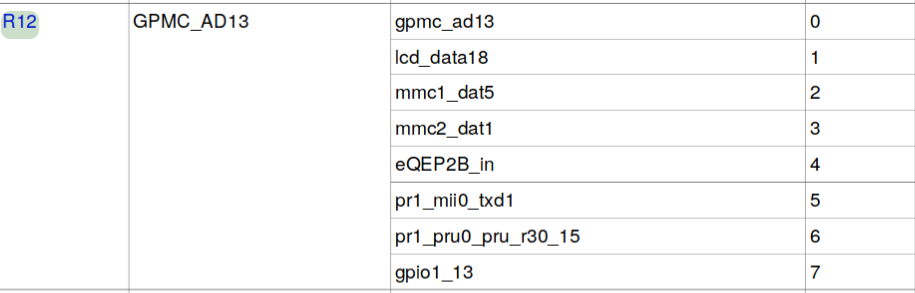
\includegraphics[width=5in]{IMAGES/p233-zcz-r12}
		     \caption{P2.33 ZCZ R12 (gpio1\_13)}
	     \end{figure}
\end{frame}

\begin{frame}
    {Describing the Joystick Hardware}
\begin{itemize}
	\item
		Specify the MMA8453 accelerometer
	\item
		Specify the Left and Right buttons used by joystick
	\item
		Specifiy the MMA8453 channels used by joystick
	\item
		Specify pinmux settings needed for buttons
	\item
		Specify GPIO resources needed for buttons
\end{itemize}
\end{frame}

\begin{frame}
    {Joystick DT Overlay}

	\begin{raw}
/dts-v1/;
/plugin/;

#include <dt-bindings/gpio/gpio.h>

/ {
        fragment@0 {
                target = <&i2c2>;
                __overlay__ {
                        #address-cells = <1>;
                        #size-cells = <0>;
                        mma8453: mma8453@1c {
                                #io-channel-cells = <1>;
                                status = "okay";
                                compatible = "fsl,mma8453";
                                reg = <0x1c>;
                        };

                };
        };
	\end{raw}
\end{frame}

\begin{frame}
	{Joystick DT Overlay (continued)}

	\begin{raw}
        fragment@1 {
                target = <&ocp>;
                __overlay__ {
                        P2_33_pinmux { status = "disabled"; };  /* Left - gpio3_21 */
                        P1_29_pinmux { status = "disabled"; };  /* Right - gpio1_13 */
                        cape-universal { status = "disabled"; };

                        joystick {
                                compatible = "bborg,techjoy";
                                pinctrl-0 = <&P2_33_gpio_input_pin>,
                                            <&P1_29_gpio_input_pin>;
                                io-channels = <&mma8453 0>, <&mma8453 1>;
                                io-channel-names = "accel_x", "accel_y";
                                button-gpios = <&gpio3 21 GPIO_ACTIVE_LOW>,
                                               <&gpio1 13 GPIO_ACTIVE_LOW>;
                        };
                };
        };
};
	\end{raw}
\end{frame}

\begin{frame}
	{Build/Install joystick overlay}
	\begin{raw}
# cp techjoy.dts /opt/source/bb.org-overlays/src/arm/
# cd /opt/source/bb.org-overlays
# make src/arm/techjoy.dtbo
# make install
	\end{raw}
\end{frame}

\begin{frame}
	{Deploy joystick overlay}

	Edit \textbf{/boot/uEnv.txt} disabling/enabling overlays as follows:
	\begin{raw}
#uboot_overlay_addr0=/lib/firmware/PB-I2C2-ACCEL-TECHLAB-CAPE.dtbo
#uboot_overlay_addr1=/lib/firmware/PB-PWM-RGB-TECHLAB-CAPE.dtbo
#uboot_overlay_addr2=/lib/firmware/PB-SPI1-7SEG-TECHLAB-CAPE.dtbo
#uboot_overlay_addr3=/lib/firmware/PB-SPI0-OLEDC-CLICK.dtbo
uboot_overlay_addr0=/lib/firmware/techjoy.dtbo
	\end{raw}

	Reboot the board to activate the overlay:
	\begin{raw}
# reboot
	\end{raw}
\end{frame}
